\documentclass[11pt]{article}
\usepackage{amsmath,textcomp,amssymb,geometry,graphicx,tikz,cancel}
\usepackage{algpseudocode,algorithm}
\usepackage[T1]{fontenc}
\usepackage[colorlinks=true,urlcolor=blue]{hyperref}

\def\Name{Zackery Field}  % Your name
\def\Sec{}  % Your GSI's name and discussion section
\def\Login{} % Your login
\def\Homework{1}%Number of Homework
\def\Session{Spring 2014}

\title{Lab 4: Protein Structure Visualization}
\author{\Name}%, section \Sec, \texttt{\Login}}
\markboth{--\Session\  Homework \Homework\ \Name, section \Sec}
{\Session\ Homework \Homework\ \Name, section \Sec, \texttt{\Login}}
%\pagestyle{myheadings}

\begin{document}
\maketitle

\section*{Part 1.   Identifying proteins from PDB}

\begin{itemize}
\item[1E9R:] Images 1 and 2
\item[4AT1:] Image 3
\item[1AON:] Images 4 and 5
\item[1BL8:] Images 6 and 7
\item[1MSL (2OAR):] Image 8
\item[2POR:] Image 11
\item[2JK2:] Image 9
\item[1ID1:] Image 10
\item[2WFH:] Image 12
\item[3CEQ:] Image 13
\end{itemize} 

\section*{Part 2. Active site images of Human Carbonic Anhydrase II}

Human Carbonic Anhydrase II

PDB ID: 1MOO

EC Number: 4.2.1.1

\href{http://www.ebi.ac.uk/intenz/query?cmd=SearchID&id=4662}{CAS link}

\begin{figure}

  \centering

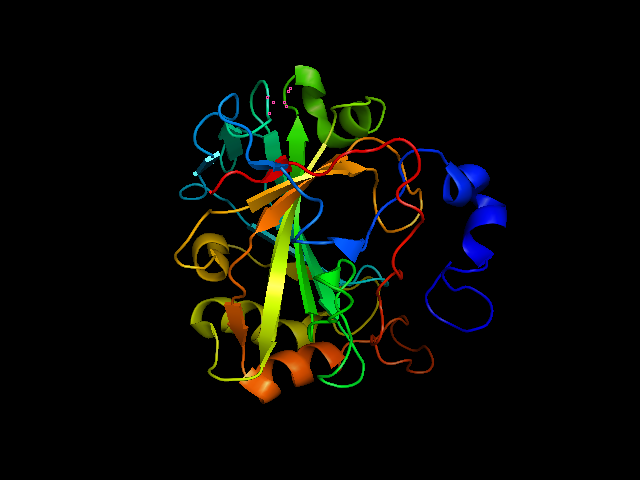
\includegraphics[scale=0.5]{1MOO_whole.png}

\caption{An overview image of the structure of 1MOO. 1MOO is a Human Carbonic Anhydrase}
\end{figure}


This anhydrase is present in humans. It plays a major role in maintaining acid-base
equilibrium in blood by converting carbonic acid to water and carbon dioxide. This 
type of enzyme has very high activity, and is usually limited by the diffusion of its
substrates. Neighboring the third histidine residue mentioned in Figure 2 is
a water molecule forms the final position necessary to sequester the zinc ion.
This water molecule is also polarized by the presence of the zinc ion. 
Not pictured in the second figure is a fourth histidine residue that
accepts a proton from water. \href{http://en.wikipedia.org/wiki/Carbonic_anhydrase}{Source}


\begin{figure}
  \centering 

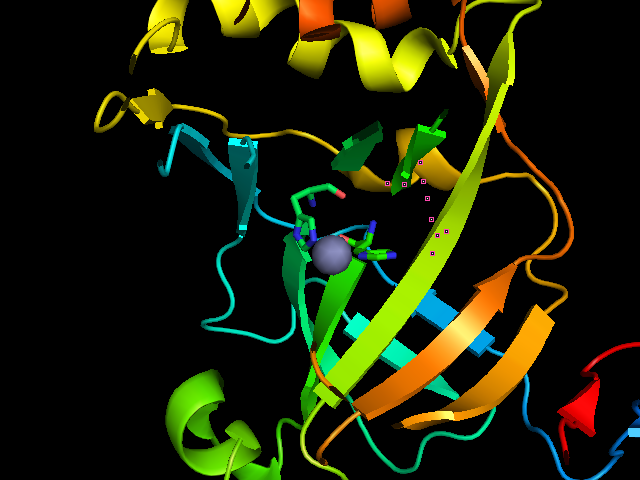
\includegraphics[scale=0.5]{1MOO_active.png}

\caption{This image highlights the active site region, and cofactor sites of Human
Carbonic Anhydrase II. The grey sphere represents the zinc cofactor located at the
active site. The residues in "stick" representation are two of the three hitidine residues
that hold the zinc ion in place at the active site.
}
\end{figure}

\end{document}